\documentclass[10pt,a4paper]{article}


\usepackage[T1]{fontenc}
\usepackage[utf8]{inputenc}
\usepackage[english]{babel}
\usepackage[english]{isodate}
\usepackage[parfill]{parskip}
\usepackage[margin=3.cm]{geometry}
\usepackage{graphicx}
\graphicspath{{./figs/}}
\usepackage{amsmath}
\usepackage{amssymb}
\usepackage{cite}

\usepackage{xcolor}
\usepackage[caption=false]{subfig}
\usepackage{caption}
%\usepackage{orcidlink}
\usepackage{hyperref}
\hypersetup{
	colorlinks = true,
	urlcolor   = blue,
	citecolor  = black,
	linkcolor = black
}

\title{MyPTV user manual}
\author{Ron Shnapp\footnote{ronshnapp@gmail.com}}
\date{\today\\[.3cm] Version 0.1}

\begin{document}
	
\maketitle

\pagenumbering{Roman}
\tableofcontents
\newpage

\pagenumbering{arabic}







\section{3D-PTV principles}


The 3D-PTV method is used to measure trajectories of particles in 3D space. It utilises the pronciples of stereoscopic vision in order to reconstruc 3D positions of particles from images taken from several angles. A scheme of a typical 3D-PTV experiment using a four camera system is shown in Fig.~\ref{fig:3dptv_exp}. The "work horse" behind the 3D-PTV method is the colinearity condition, the 3D model. In principle, if we know what is the position and what is the orientation of the camera in 3D space ($O'$ and $\theta$ in Fig.~\ref{fig:3dmodel}), we can use the pin-hole camera model to relate the image space coordinates of a particle ($\eta,\, \zeta$ in Fig.~\ref{fig:3dmodel}) to the ray of light connecting the imaging center and the particle. Then, if we have more than one camera, the particle will be located at the intersection of the two rays. Detailed information is given in \cite{Virant1997, Mass1993}.  


\begin{figure}[h!]
	\centering
	\subfloat[]{\label{fig:3dptv_exp}
		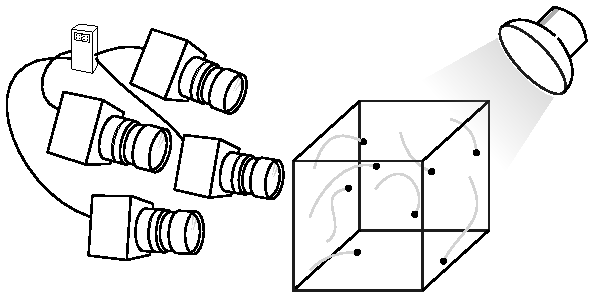
\includegraphics[width=6.5cm]{3D_PTV_acquisition.pdf}}
	\hfill
	%
	\subfloat[]{\label{fig:3dmodel}
		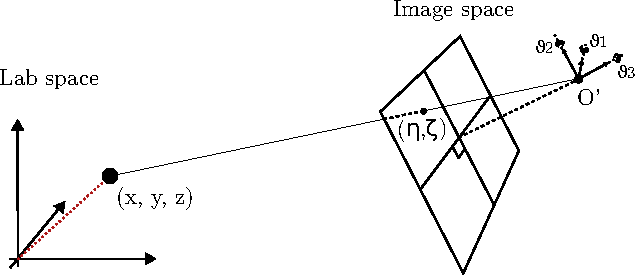
\includegraphics[width=6.5cm]{pinhole_model.pdf}}
	%
	\caption{(a) A schematics of a 3D-PTV experiment. (b) A schematic description of the 3d model, the pin-hole camera model.}
\end{figure}



Once the experiment, namely data aquisition, is done, there are six intrinsic steps to follow in order to complete the analysis. The six steps are outlined in Fig.~\ref{fig:steps}. In Camera calibration, we use images of known calibration targets to estimate the position, orientation and internal parameters of the cameras. In particle segmentation we use image analysis to obtain the paritlces' image space coordinates ($\eta, \, \zeta$). In the Particle matching step we use the ray crossing principle to decide which particle image in each of the cameras correspond to the same physical particle, and triagulate their positions through stereo mathcing. In particle tracking we connect the positions of particles in 3D space to form trajectories. In data conditioning we might use smoothing and re-tracking algorithms to enhance the quality of our data according to some physical heuristics. Lastly, we can analyze the data to obtain information on the physics of the particles we are studying. The MyPTV package is meant to handle the first five of these steps.    



\begin{figure}
	\centering
	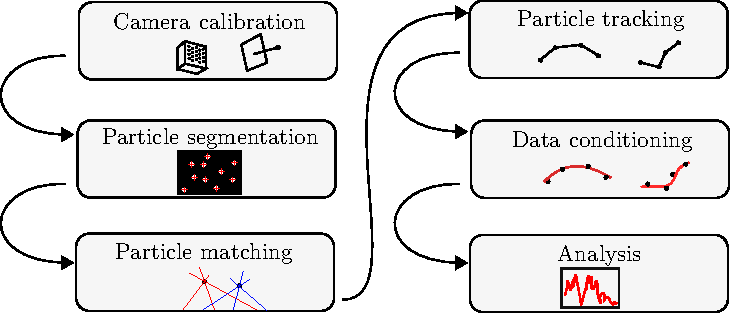
\includegraphics[width=10cm]{steps.pdf}
	\caption{Basic steps in the analysis of PTV raw data into particl trajectories and scientific output. The first five steps are handled by MyPYV. \label{fig:steps}}
\end{figure}


The sections that follow outline the code used to handle the 3D-PTV method in MyPTV.







\section{Imaging module - \texttt{imaging\char`_mod.py}}


The imaging module is used to handle the translation from 2D image space coordinates to lab spcae coordinates and vice-versa. For that, we use the following mathematical model:
%
\begin{equation}
\vec{r}-\vec{O} = \Big( \, 
\begin{bmatrix}
\eta + x_h\\
\zeta + y_h \\
f
\end{bmatrix}
+ \vec{e}(\eta, \zeta) \,\Big) \cdot \Big[ R \Big]
\label{eq:3dmodel}
\end{equation}
%
where the description of the notations is given in Table~\ref{tab1:mathdesc}. The matrix $[R]= [R_1]\cdot [R_2] \cdot [R_3]$ is the rotation matrix calculated with the components of the orientation vector, $\vec{\theta} = [\theta 1,\, \theta 2,\, \theta 3]$. In addition, the correction temr $\vec{e}$ is assumed to be a quadratic polynomial of the image space coordinates:
%
\begin{equation}
\vec{e}(\eta,\,\zeta) = [E]\cdot P(\eta,\,\zeta) =
\begin{bmatrix}
E_{11} & E_{12} & E_{13} & E_{14} & E_{15}\\
E_{21} & E_{22} & E_{23} & E_{24} & E_{25}\\
0 & 0 & 0 & 0 & 0
\end{bmatrix}
\cdot 
\begin{bmatrix}
\eta\\
\zeta\\
\eta^2\\
\zeta^2\\
\eta\,\zeta
\end{bmatrix}
\end{equation}
%
where $[E]$ is a $3\times5$ matrix that holds the correction coefficients; the last row is filled with zeros because we do not attempt to correct $f$.





\begin{table}
	\centering
	\caption{Description of mathematical notation. \label{tab1:mathdesc}}
	\begin{tabular}{p{5em} p{30em}}
		 \hline
		Symbol & Description \\ \hline
		$\vec{r}$ & Particle position in the lab space coorindates\\
		$\vec{O} $& Position of a camera's imaging center \\
		$\eta, \, \zeta$ & image space coordinates (pixels) of a particle \\
		$x_h , \, y_h$ & Correction to the camera's imaging center (in pixels)\\
		$f$ & The camera's principle distance divided by the pixel size \\ 
		$\vec{e}(\eta, \zeta)$ & A nonlinear correction term to compensate for image distortion and multimedia problems.\\
		$[R]$ & The roation matrix which corresponds to the camera orientation vector. \\  \hline
	\end{tabular}
\end{table}






\subsection{The \texttt{camera} object}\label{sec:camera}

An object that stores the camera external and internal parameters and handles the projections to and from image space and lab space. Inputs are:

\begin{enumerate}
	\item \texttt{name} - string, name for the camera. This is the name used when saveing and loading the camera parameters.
	\item \texttt{resolution} - tuple (2), two integers for the camera number of pixels
	\item \texttt{cal\char`_points\char`_fname} - string (optional), path to a file with calibration coordinates for the camera. The format fro the calibration point file is given in Section~\ref{sec:calpointreader} (see Fig.~\ref{fig:calpointfile}).
\end{enumerate}


The important functionalities are:


\begin{enumerate}
	\item \texttt{get\char`_r(eta, zeta)} - Will solve eq.~\ref{eq:3dmodel} for the orientation vector $\vec{b} = \vec{r} - \vec{O}$, given an input of pixel coordinates $(\eta, \, \zeta)$.
	
	\item \texttt{projection(x)} - Will reverse solve equation~\eqref{eq:3dmodel} to find the image space coordinates $(\eta, \, \zeta)$, of an input 3D point, (\texttt{x=}$\vec{r}$).
	
	\item \texttt{save(dir\char`_path)} - Will save the camera parameters in a file called after the camera name in the given directory path, see Fig.~\ref{fig:camfiles}.
	
	\item \texttt{load(dir\char`_path)} - Will load the camera parameters in a file called after the camera name in the given directory path, see Fig.~\ref{fig:camfiles}.
\end{enumerate}



After calibration we can save the camera parameters on the hard disc. The camera files have the structure shown in Fig.~\ref{fig:camfiles}.

\begin{figure}
	\centering
	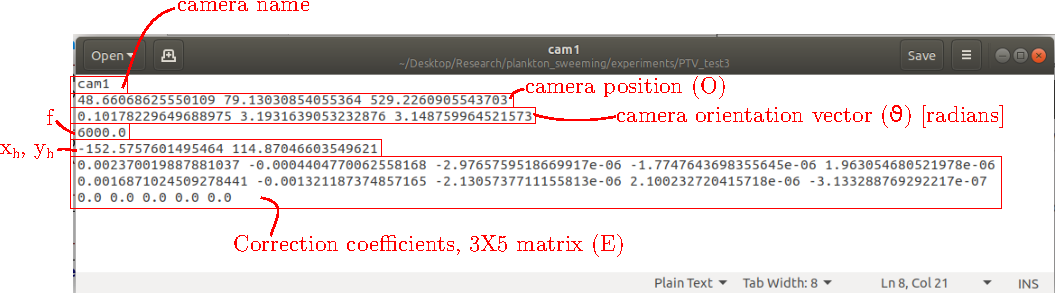
\includegraphics[width=\textwidth]{camera_files.pdf}
	\caption{The structure of a camera file. The files are simple text files where each row corresponds to a specific paramter and the values in each row are separated by a whitespace. \label{fig:camfiles}}
\end{figure}








\subsection{The \texttt{imsys} object}


An object that holds several camera instances and can be used to perform stereo-matching. The important functionalities are:


\begin{enumerate}
	\item \texttt{stereo\char`_match(coords, d\char`_max)} - Takes as an input a dicionary with coordinates in image space from the several cameras and calculates the triagulation position. \\ The coordinate dicitonary has keys that are the camera number and the values which are the coordinates in each camera. d\char`_max is maximum allowable distance for the triangulation.
	
\end{enumerate}








\subsection{The \texttt{Cal\char`_image\char`_coord} object}\label{sec:calpointreader}

This is a class used for reading information given in the optional argument \texttt{cal\char`_points\char`_fname} of the \texttt{camera} class (Sec.~\ref{sec:camera}). It is used internally and generally users will not have to deal with this. This class will read and interpret text files with tab separated valued, where the columns' meanings are: [x image space, y image space, x lab space, y lab space, z lab space], and each row is a single point of some known calibration target.

The input for this class is:
\begin{enumerate}
	\item \texttt{fname} - String, the path to your calibration point file. The file is holds tab separated values with the meaning of: [x image, y image, x lab, y lab, z lab], see Fig.~\ref{fig:calpointfile}.
\end{enumerate}



\begin{figure}
	\centering
	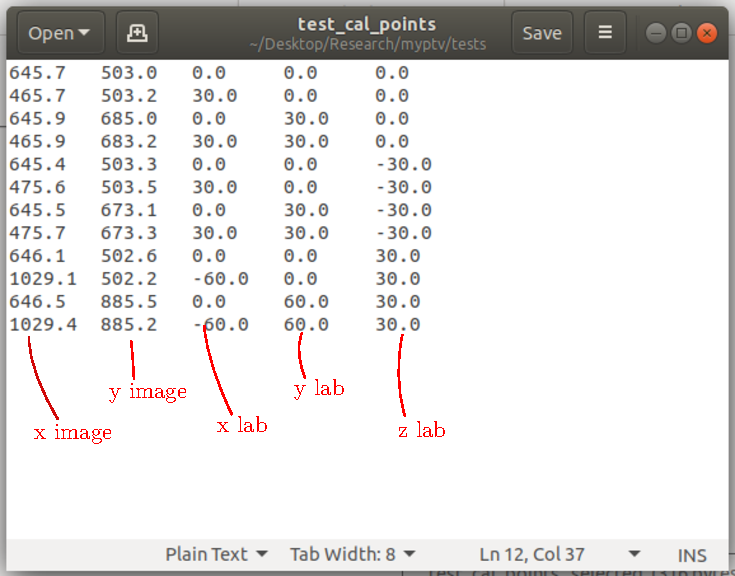
\includegraphics[width=10cm]{cal_point_file.pdf}
	\caption{An example of a text file holding the calibration point data. \label{fig:calpointfile}}
\end{figure}





\section{Camera calibration - \texttt{calibrate\char`_mod.py}}


Holds the \texttt{calibrate} object that is used to find the camera calibration parameters.



\subsection{The \texttt{calibrate} object}

Used to solve for the camera parameters given an input list of image space and lab space coordinates. The inputs are:

\begin{enumerate}
	\item \texttt{camera} - An instance of a \texttt{camera} object which we would like to calibrate.
	\item \texttt{lab\char`_coords} - a list of lab space coordinates of some known calibration target. 
	\item \texttt{img\char`_coords} - a list of image space coordinates that is ordered in accordance with the lab space coordinates. 
\end{enumerate}



The important functionalities are:
%
\begin{enumerate}
	
	\item \texttt{searchCalibration(maxiter=5000, fix\char`_f=True)} - When this is run, we use a nonlinear least squares search to find the camera parameters that minimize the cost function (item 3 below). This function is used to find the $\vec{O}$, $\vec{\theta}$, $f$, and $x_h, \, y_h$ parameters (in case \texttt{fix\char`_f=False}, it will not solve for $f$. \texttt{maxiter} is the maximum number of iterations allowed for the least squares search.
	
	\item \texttt{fineCalibration(maxiter=500)} - This function will solve for the coefficients of the quadratic polynomial used for the nonlinear correction term ($[E]$). 
	
	\item \texttt{mean\char`_squared\char`_err} - This is our cost function, being the sum of distances between the image space coordinates and the projection of the given lab space coordinates.
	
\end{enumerate}
%
To find an optomal calibration solution, we might need to run each function several times, and run the coarse and fine calibrations one after the other until a satisfactory solution is obtained. Once it is obtained, we should keep in mind to save the results using the \texttt{save} functionality of the \texttt{camera} object. 








\section{Particle segmentation - \texttt{segmentation\char`_mod.py}} 


This module handles the image analysis part of MyPTV, taking in raw camera images containing particles and outputing their image space coordinates. For the segmentation we first blur the image to remove salt and pepper noise, then we highlight particles using a local mean subtraction around each pixel, and then use a global threshold to mark foreground and backgroud pixels. Finally, the connected foreground pixels are considered to be particles, and we estimate the blob's center using a brightness weighted average of blob pixels.



\subsection{The \texttt{particle\char`_segmentation} object} 

Used to segment particles in a given image. This class is used internally to iterate over frames in a single folder by the \texttt{loop\char`_segmentation} class. However, it is usefull to check the segmentation parameters manually using this \texttt{particle\char`_segmentation} over several images in order to tune the particle searching. The inputs are:
%
\begin{enumerate}
	\item \texttt{image} - the image for segmentation
	\item \texttt{sigma=1.0} - the standard deviation of the blurring filter
	\item \texttt{threshold=10} - the global filter's threshold brightness value (pixels with brightness higher than this number are considered foreground) 
	\item \texttt{mask=1.0} - A mask matrix can be used to specify rigions of interest within the image
	\item \texttt{local\char`_filter=15} - The window size (pixels) for the local filter.
	\item a bunch of threshold pixel sizes in all directions and in area.
\end{enumerate}


The important funcitonalities are:
%
\begin{enumerate}
	\item \texttt{get\char`_blobs} - Will return a list of blob centers, their box size and their area.
	\item \texttt{plot\char`_blobs()} - Uses matplotlib to plot the results of the segmentation. A very usefull functionality in the testing of segmentation parameters!
\end{enumerate}






\subsection{The \texttt{loop\char`_segmentation} object} 


An object used for looping over images in a given directory to segment particles
and save the results in a file.


important functionalities are:
%
\begin{enumerate}
	\item \texttt{segment\char`_folder\char`_images()} - Will loop over the images in the given directory and segment particles according to the given parameters
	\item \texttt{save\char`_results(fname)} - Will save the segmented particles in a text file. The file is arranged in six columns with the following attributes: (x center position, y center position, x size, y size, area, image number), see Fig.~\ref{fig:blobfile}.
\end{enumerate}

\begin{figure}[h!]
	\centering
	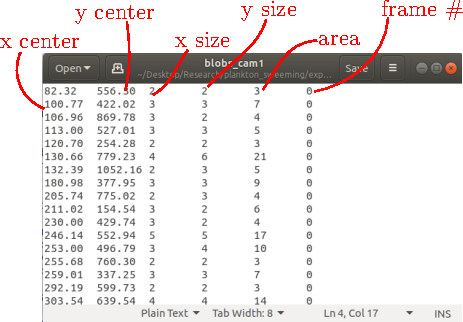
\includegraphics[width=10cm]{blob_file.pdf}
	\caption{An example of a text file holding the segmentation resuls and the description of the different columns. \label{fig:blobfile}} 
\end{figure}








\section{Particle matching - \texttt{particle\char`_matching\char`_mod.py}}

The module used to identify the same particle in the different images and use stereo matching to estimate their 3D position. Particle matching in MyPTV uses the Ray Traversal algorith proposed in Ref~\cite{Bourgoin2020}. In short, the 3D domain is divided into voxel cubes; then, for each segmented blob we shoot a ray throught the 3D volume and list the voxels through which the ray had passed. Finally, is more than one ray had passed through a certain voxel, we stereo match the blobs at the intersection. Lastly, for each stereomatched blob, we keep the particles corresponding to the highest number of cameras (for example, we favour particles that result from a crossing of four camera views than three) and the smallest RMS distance from the epipolar lines.  


\subsection{The \texttt{match\char`_blob\char`_files} object}


This is the object that we use in order to obtain trangulated particles results from the segmented blob files (a file as the one in Fig.~\ref{fig:blobfile} for each camera). The inputs are:
%
\begin{enumerate}
	\item \texttt{blob\char`_fnames} - a list of the (srting) file names containing the segmented blob data. The list has to be sorted according the order of cameras in the \texttt{img\char`_system}.
	\item \texttt{img\char`_system} - an instance of the \texttt{img\char`_system} class with the calibrated cameras.
	\item \texttt{RIO} - A nested list of 3X2 elements. The first holds the minimum and  maximum values of $x$ coordinates, the second is same for $y$, and  the third for $z$ coordinates. 
	\item \texttt{voxel\char`_size} - the side length of voxel cubes used in the ray traversal algorithm. Given in lab space coordinates (e.g. mm).
	\item \texttt{max\char`_err=None} - Maximum acceptable uncertainty in particle position. If None, (defult), than no bound is used.
	\item \texttt{reverse\char`_eta\char`_zeta=False} - Should be false if the eta and zeta coordinates need to be in reverse order so as to match the calibration. This may be needed if the calibration data points were given where the x and y coordinates are transposed (as happens, e.g., if using matplotlib.pyplot.imshow).
\end{enumerate}


The important functionalities are:
%
\begin{enumerate}
	\item \texttt{get\char`_particles()} - Use this to match blobs into particlesin 3D.
	\item \texttt{save\char`_results(fname)} - Save the results in a text file. The format has 4 + number of cameras columns separated by tabs:
	(x, y, z, [N columns corresponding to the blob number in each camera] , frame number, see Fig.~\ref{fig:particlefile}).
\end{enumerate}



\begin{figure}[h!]
	\centering
	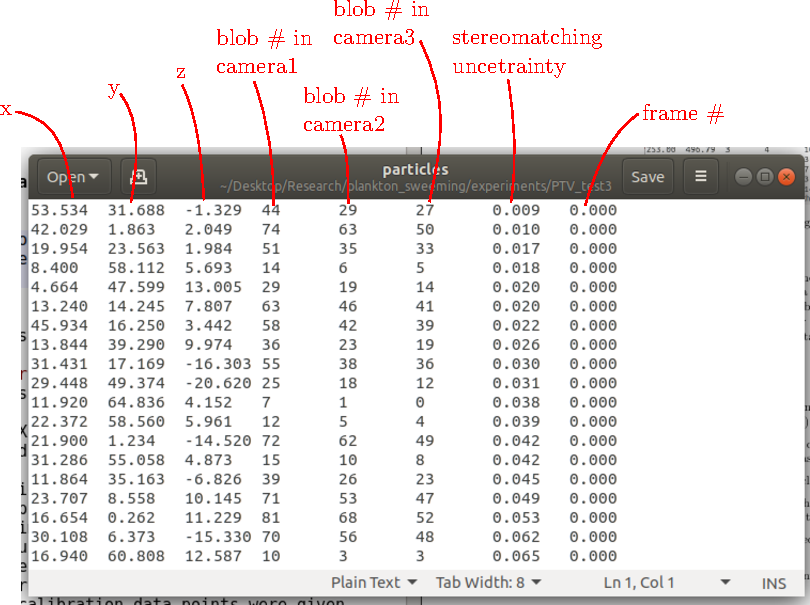
\includegraphics[width=12cm]{particle_file.pdf}
	\caption{An example of a text file holding the triangulated particles' resuls and the description of the different columns. In this example there were three cameras. \label{fig:particlefile}} 
\end{figure}




\subsection{The \texttt{matching} object}

This object is the engine used backstage for matching particles. In practice we run the relevant functions: \texttt{get\char`_voxel\char`_dictionary()} $\rightarrow$ \texttt{list\char`_candidates()} $\rightarrow$ \texttt{get\char`_particles()}, and after that the results are held in the attribute \texttt{matched\char`_particles}.








\section{Tracking in 3D - \texttt{tracking\char`_mod.py}}

This is the module that is used to track particles in 3D. There are currently three tracking methods implemented, nearest neighbour, two-frame, and four-frame, see Ref.~\cite{Ouellette2006}. Users are welcome to choose their perfered method and use it.



\subsection{The \texttt{tracker\char`_four\char`_frames} object}\label{sec:four_frames}

An object used to perform tracking through the 4-frame best estimate method \cite{Ouellette2006}. Input:
%
\begin{enumerate}
	\item \texttt{fname} - a string name of a particle file (e.g. Fig.~\ref{fig:particlefile}
	\item \texttt{mean\char`_flow=0.0} - either zero (deafult) of a numpy array of the mean flow vector, in units of the calibrations spatial units per frame (e.g. mm per frame). The mean flow is assumed not to change in space and time.
	\item \texttt{d\char`_max\char`=1e10} - maximum allowable translation between two frames for the nearest neighbour search, after subtracting the mean flow. 
	\item \texttt{dv\char`_max\char`=1e10} - maximum allowable change in velocity for the two-frame velocity projection search. The radius around the projection is therefore dv\char`_max/dt (where dt = 1 frame$^{-1}$)
\end{enumerate}


The important functionalities are:
%
\begin{enumerate}
	\item \texttt{track\char`_all\char`_frames()} - Will track particles through all the frames. 
	
	\item \texttt{return\char`_connected\char`_particles()} - Will retun the list of trajectories that were established.
	
	\item \texttt{save\char`_results(fname)} - Will save the results on the hard drive. The results are saved in a text file, where each row is a sample of a trajectory. The columns are specified as follows: [trajectory number, x, y, z, frame number], see Fig~\ref{fig:trajfile}.  
\end{enumerate}

\begin{figure}
	\centering
	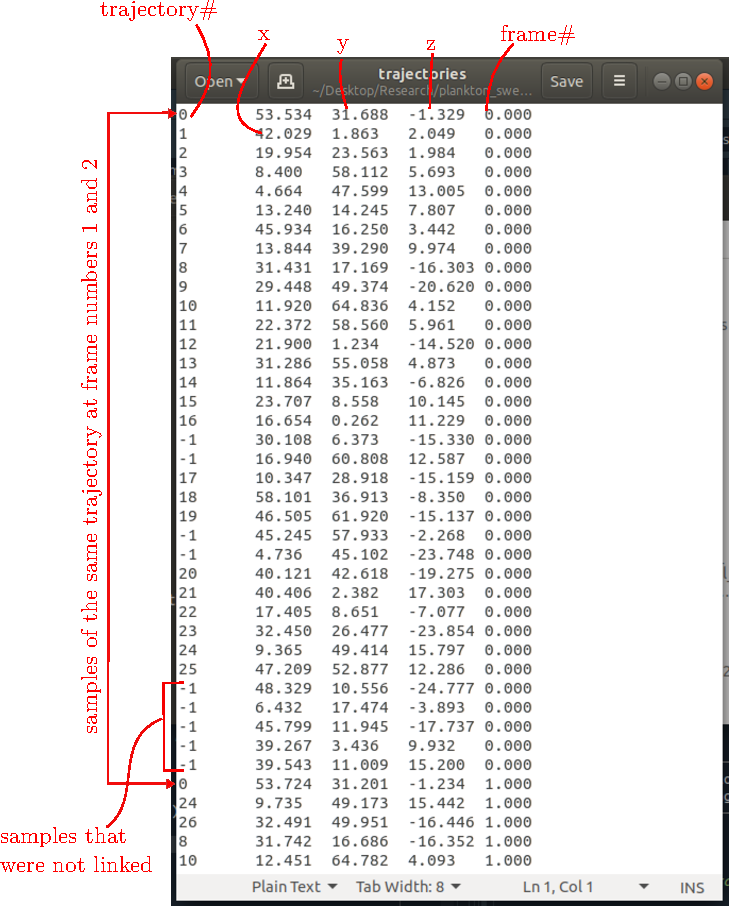
\includegraphics[width=10cm]{trajectory_files.pdf}
	\caption{Example of a trajectory file and the column definitions. \label{fig:trajfile}}
\end{figure}




\subsection{The \texttt{tracker\char`_two\char`_frames} object}

An object used for tracking through the 2-frame method. The description is the same as in Section~\ref{sec:four_frames}



\subsection{The \texttt{tracker\char`_nearest\char`_neighbour} object}

An object used for tracking through the nearest neighbour method. The description is the same as in Section~\ref{sec:four_frames}









\section{Trajectory smoothing - \texttt{traj\char`_smoothing\char`_mod.py}}

This module is used to smooth trajecotries and to calculate the velocity and acceleration of the particles. For the smoothing we are using the polynomial fitting methd proposed and used in Refs.~\cite{Luthi2005, Shnapp2019}. In short, each component of the particle's position is fitted with a series of polynomials with a sliding window of fixed lenght and the derivatives are calculated by analytically differentiating the polynomial. The end result is a new file with smoothed trajectories. However note that we smooth and calculate valocities and accelerations only for trajectories longer than the window size for the smoothing (a user decided parameter). 


\subsection{The \texttt{smooth\char`_trajectories} object}

A class used to smooth trajectories in a list of trajectories. Due to the smoothing we also calculate the velocity and acceleration of the trajectories. The input trajecotry list structure is the same as the files produced by the classes in \texttt{tracking\char`_mod.py}.

Note - only trajectories whose length is larger than the window size will be smoothed and saved. Shorter trajectories are svaed with zero velocity and accelerations.


The inputs are:
\begin{enumerate}
	\item \texttt{traj\char`_list} -  a list of samples organized as trajecotries. This should have the same data structure used in the saving function of the tracking algorithms (see Section~\ref{sec:four_frames}). 
	\item \texttt{window} - The window size used in the sliding polynomial fitting.
	\item \texttt{polyorder} - The order of the polynomial used in the fitting. 
\end{enumerate}

\begin{figure}[h!]
	\centering
	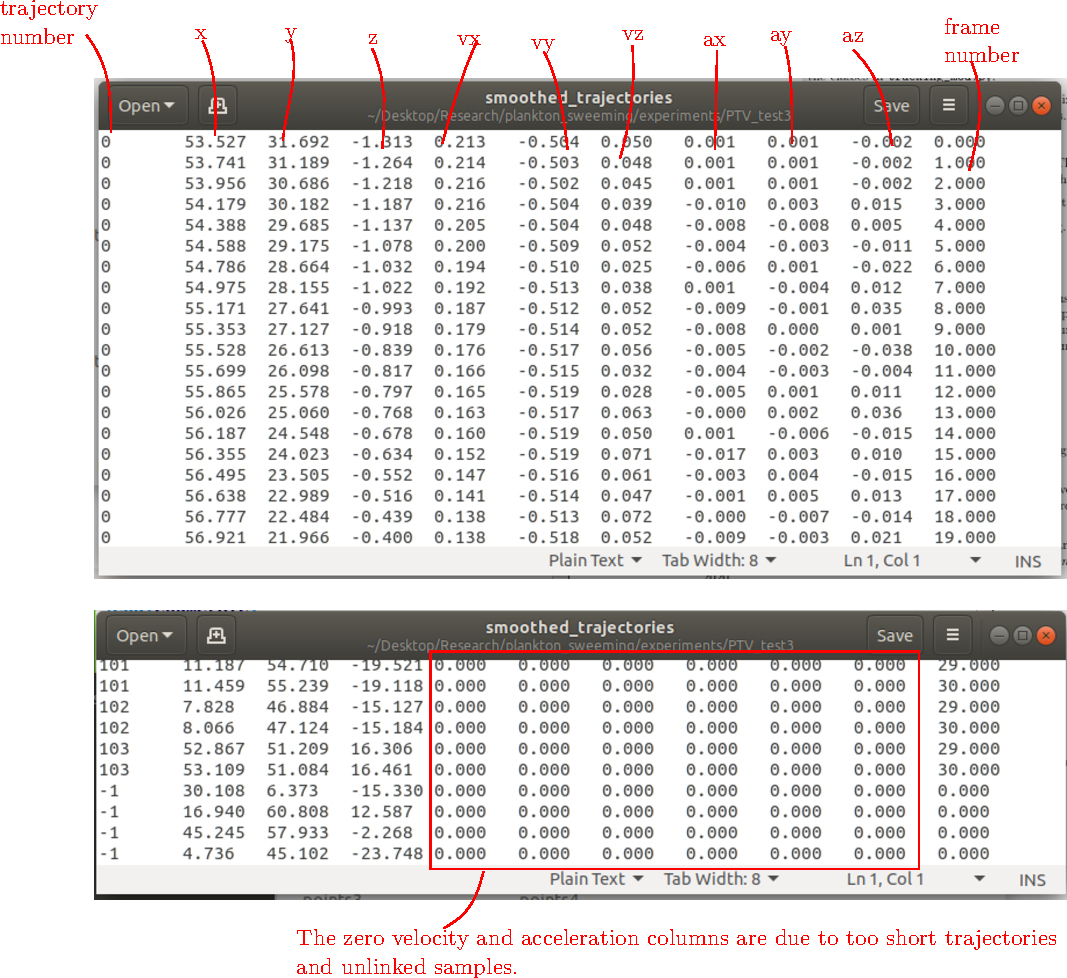
\includegraphics[width=12cm]{smoothed_trajfile.pdf}
	\caption{Example file holding the results of smoothed trajectories, and the description for each column. Note also the unsmoothed samples at the bottom of the file. \label{fig:smoothedfile}}
\end{figure}

The important functionalities are:

\begin{enumerate}
	\item \texttt{smooth()} - performs the actual smoothing
	\item \texttt{save\char`_results(fname)} - Saves the results on the hard drive using the given (string) file name. The resulting file is a text file such that each row is a sample of a trajectory, and with 11 columns. The columns have the following meaning:
	[traj number, $x$, $y$, $z$, $v_x$, $v_y$, $v_z$, $a_x$, $a_y$, $a_z$, frame number], where $v_i$ and $a_i$ denote components of the velocity and acceleration vectors respectively, see Fig.~\ref{fig:smoothedfile}.
\end{enumerate}





\bibliography{bib_myPTV}
\bibliographystyle{unsrt}

\end{document}